\section{Séance 3 : Feed-Forward}
\subsection{Introduction}
Le but de la séance est d'utiliser la technique du \textbf{feed-forward}. Une action de ce type, si elle bien paramétrées, rend invisibles une perturbation pour la sortie du système.La perturbation étudiée sera un changement de vitesse du ventilateur. Elle se présentera sous la forme d'un échelon 50 à 60\% de la vitesse maximale dudit ventilateur.\\

Pour paramétrer ce type d'action, il est primordial d'avoir un régulateur optimisé. Sur base des essais réalisés au dernier laboratoire, plusieurs groupes de paramètres ont été testés pour tendre vers un régulateur efficace. Pour ce faire, il a été choisi de partir du régulateur testé lors de l'essai 1 de la première séance. À partir de ces paramètres, nous avons abouti sur un régulateur optimisé. Les résultats de cette démarche seront présentés sous forme d'une \textit{feuille de résultat} comprenant :
\begin{itemize}
\item Le graphe de la sortie du système 
\item Le graphe de la consigne de courant appliquée par le régulateur.
\item Les valeurs de constantes utilisées.
\item Les commentaires influençant le choix des constantes de l'essai suivant.
\end{itemize}

Lorsque l'on désire paramétrer une action en feed-forward, il est nécessaire de connaitre la fonction de transfert de la perturbation. Celle-ci sera obtenue au moyen d'un programme d'optimisation. Le point \ref{FW} détaillera de manière plus précise la manière d'utiliser ce type d'action.\\ 


\subsection{Optimisation du régulateur}
\begin{optibox}{essai1}{6}{150}{15}
On peut observer que la consigne de courant sature. De ce fait, on observe que le système tend vers la consigne mais en oscillant.  Il a été décidé de réaliser l'essai suivant en augmentant la valeur de la constante proportionnelle.
\\\hline
\end{optibox}
\
begin{optibox}{essai2}{10}{150}{15}
La consigne de courant sature encore plus.
Cependant, les essais 3 à 12 ne seront pas présentés car ils sont contre-productifs. Une mauvaise compréhension de certains paramètres nous ont conduits à augmenter la valeur de $K_{p}$ jusque 30. Voyant que nous nous écartions d'une régulation efficace, il a été convenue de repartir de l'essai 1 pour poursuivre l'optimisation mais en diminuant seulement la valeur de $T_{d}$\\
\hline
\end{optibox}

\begin{optibox}{essai13}{6}{150}{8}
La consigne de courant ne sature plus mais on observe un grand dépassement. Les valeurs de $K_{p}$ et $T_{d}$ seront donc diminué pour l'essai suivant. La consigne n'étant pas atteinte après 270 secondes, l'essai a été avorté. 
\\\hline
\end{optibox}

\begin{optibox}{essai14}{4}{80}{8}
La consigne de température étant atteinte et le dépassement étant faible, la composante intégrative sera diminuée et le facteur de dérivation sera quant à lui augmenté pour essayer d'accélérer la régulation du système.
 \\\hline
\end{optibox}

\begin{optibox}{essai15}{4}{65}{10}
La consigne de température est atteinte en deux oscillations et en 200 secondes. Pour diminuer l'oscillation on augmente encore le  $T_{d}$. On augmentera aussi un tout petit peu le facteur proportionnel pour diminuer en même temps le dépassement.\\\hline
\end{optibox}

\begin{optibox}{essai16}{4.5}{65}{15}
La sortie du système ne présente plus de dépassement mais la consigne est atteinte plus lentement qu'à l'essai précédent. La valeur de $T_{d}$ sera légèrement diminuée.
\\\hline
\end{optibox}

\begin{optibox}{essai17}{4.5}{65}{12.5}
Le dépassement est très faible et la température souhaitée est atteinte en moins de 200 secondes. 
Les paramètres de cet essai seront utilisés pour comme constante du régulateur optimisé.
\\\hline
\end{optibox}


%DATA.
%\begin{itemize}
%\item $K_{p} = 20$, $T_{i} = 150$ et $T_{d} = 15$(4)
%\item $K_{p} = 15$, $T_{i} = 150$ et $T_{d} = 7$(5)
%\item $K_{p} = 10$, $T_{i} = 150$ et $T_{d} = 7$(6)
%\item $K_{p} = 10$, $T_{i} = 150$ et $T_{d} = 11$(7)
%\item $K_{p} = 12$, $T_{i} = 100$ et $T_{d} = 13$(8)
%\item $K_{p} = 17$, $T_{i} = 100$ et $T_{d} = 13$(9)
%\item $K_{p} = 20$, $T_{i} = 100$ et $T_{d} = 10$(10)
%\item $K_{p} = 25$, $T_{i} = 80$ et $T_{d} = 12$(11)
%\item $K_{p} = 35$, $T_{i} = 80$ et $T_{d} = 12$(12)
%\item $K_{p} = 6$, $T_{i} = 150$ et $T_{d} = 8$(13)\\
%\item $K_{p} = 4$, $T_{i} = 80$ et $T_{d} = 8$(14)
%\item $K_{p} = 4.5$, $T_{i} = 65$ et $T_{d} = 10$(15)
%\item $K_{p} = 4.5$, $T_{i} = 65$ et $T_{d} = 15$(16)
%\item \textbf{\textcolor{green}{$K_{p} = 4.5$, $T_{i} = 65$ et $T_{d} = 12.5$}}(17)
%\end{itemize}

\subsection{Fonction de transfert}
\subsubsection{Fonction de transfert du système}
\begin{center}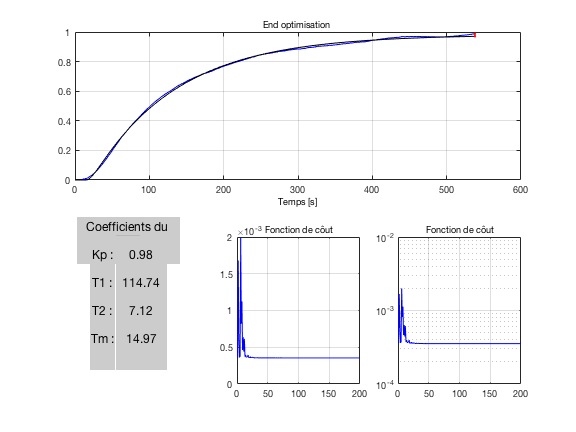
\includegraphics[scale=0.8]{optimisation/H1.png}\end{center}
\subsubsection{Fonction de transfert de la perturbation}
\begin{center}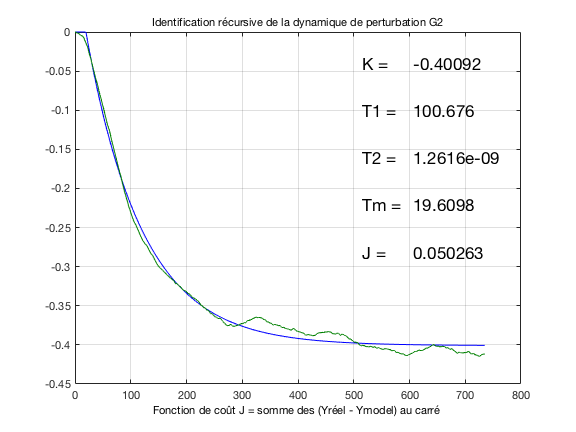
\includegraphics[scale=0.8]{optimisation/H2.png}\end{center}

\subsection{Manipulation - Feed-Forward}
\label{FW}
Vitesse du ventilateur vu comme une perturbation  qui va affecter la sortie du système. La sortie est donc une combinaison de l'influence du courant dans la résistance chauffante et de la vitesse du ventilateur (avec sa dynamique propre - cela implique une fonction de transfert)\\

Le but est de compenser la perturbation de la vitesse du ventilateur en jouant sur le courant dans la résistance (en appliquant l'inverse de la fonction de la perturbation. Dans ce cas, la perturbation serait invisible sur la sortie\\

Pour pouvoir implémenter cette solution, on a besoin de mesurer la perturbation. La perturbation devient une entrée pour le régulateur aussi\\

\begin{figure}
\centering
    
   \tikzstyle{block} = [draw, fill=blue!20, rectangle, minimum height=3em, minimum width=6em]
   \tikzstyle{sum} = [draw, fill=blue!20, circle, node distance=1cm]
   \tikzstyle{input} = [coordinate]
   \tikzstyle{output} = [coordinate]
   \tikzstyle{tmp} = [coordinate]
   \tikzstyle{pinstyle} = [pin edge={to-,thin,black}]

    \begin{tikzpicture}[auto, node distance=2cm,>=latex']
        % Blocks
        \node [input, name=input] {};
        \node [sum, right of=input] (sum) {};
        \node [block, right of=sum, node distance=3cm] (regulator1) {$R_{1}(s)$};
        \node [sum, right of=regulator1, node distance=3cm] (sum2) {};
        \node [block, right of=sum2, node distance=3cm] (system1) {$H_{1}(s)$};
        \node [sum, right of=system1, node distance=3cm] (sum3) {}; 
        \node [output, right of=sum3, node distance=1cm] (output) {};
		
		\node [block, above of=sum2] (regulator2) {$R_{2}(s)$};
		\node [block, above of=sum3] (system2) {$H_{2}(s)$};
		
		\node [sum, above of=system2, node distance=2cm] (sum4) {}; 
		\node [input, name=input2, above of=sum4, node distance=1cm]{}; 
		
		% Basic Flow
        \draw [->] (input) -- node [name=a] {$y_{sp}$}(sum);
        \draw [->] (sum) -- (regulator1);   
        \draw [->] (regulator1) -- (sum2);
        \draw [->] (sum2) --  node [name=e] {u}(system1);
        \draw [->] (system1) -- (sum3);
        \draw [->] (sum3) -- node [name=c] {$y_{pv}$}(output);
        
        \draw [->] (regulator2) -- (sum2);
        \draw [->] (system2) --(sum3);
        \draw [->] (sum4) -- node [name=e] {d}(system2);
        \draw [->] (input2) -- node [name=d] {$d     v_vent$}(sum4);

        \node [tmp, above of=regulator2, node distance=2cm] (link_tmp) {};
        \draw (sum4) -- (link_tmp);
        \draw [->] (link_tmp) -- node [name=e] {d} (regulator2);
        
        % feedback sum3 vers sum
        % \node [tmp, above of=regulator2, node distance=2cm] (link_tmp) {}; 
        % \node [tmp, above of=regulator2, node distance=2cm] (link_tmp) {};        
        % node[pos=0.99] {$-$}
    \end{tikzpicture}
\caption{Schéma bloc du système avec le régulateur de suivis de consigne et de réjection des perturbation}s
\end{figure}


\begin{align}
y_{pv} &= u \cdot H_{1}(s) + d \cdot H_{2}(s)\\
	   &= d \cdot R_{2} \cdot H_{1} + d \cdot H_{2}\\
	   &= d \cdot (R_{2} \cdot H_{1} + H_{2})\\
	   &= 0
\end{align}

\begin{equation}
H_{2} = R_{2} \cdot H_{1} \leftrightarrow R_{2} = \frac{-H_{2}}{H_{1}}
\end{equation}

Avec $R_{2}$ le deuxième régulateur connecté à la mesure de la perturbation et $d$ la perturbation (\textit{disturbate})

Le modèle de $H_{1}$ étant le modèle de Vander Grinten, c'est aussi le modèle que l'on va utiliser pour $H_{2}$

\begin{equation}
H_{1} =  \frac{k_{1} \cdot e^{-sT_{m1}}}{(sT_{11} + 1) \cdot (sT_{12} + 1)}
\end{equation}

\begin{equation}
H_{2} =  \frac{k_{2} \cdot e^{-sT_{m2}}}{(sT_{21} + 1) \cdot (sT_{22} + 1)}
\end{equation}


Par le schéma du système, on trouve les relations liant les fonctions de transfert et les régulateurs. On peut donc poser les relations suivantes :

\begin{align}
R_{2} &\rightarrow \frac{-k_{1}}{k_{2}} = gain\\
	  &\rightarrow e^{-s(T_{m1} - T_{m2})}\\
	  &\rightarrow \frac{(sT_{11} + 1) \cdot (sT_{12} + 1)}{(sT_{21} + 1) \cdot (sT_{22} + 1)}\\
\end{align}

Condition pour implémenter le Feed Forward
\begin{itemize}
\item Ordre de $H_{2}$ doit être égale à l'ordre de $H_{1}$
\item Le temps mort du régulateur 2 doit être plus faible que le temps de la perturbation sur la sortie (on doit calculer et agir sur la sortie au minimum en même temps que la perturbation si on veut la rendre invisible)
\item On doit pouvoir mesurer la perturbation
\end{itemize}

Le problème est que le régulateur 2 ne suit pas la consigne, il n'est la que pour rejeter la consigne. Cela implique que nous devons ajouter un régulateur pour suivre la consigne et rejeter les perturbations autres que celle mesurée. Le régulateur de suivis de consigne est celui dimensionner lors des séances précédentes. 
